\documentclass[solutions]{esg8022pset} 
  \usepackage{amsmath}
  \usepackage{amssymb}
  \usepackage{enumerate}
  \usepackage{graphicx}
  \usepackage{hyperref}
  %\usepackage{siunitx}
  \providecommand{\uvec}[1]{{\hat{\bf{#1}}}}
  \usepackage{pgf,tikz}
  \usetikzlibrary{arrows}
  \usepackage{wasysym}
  \makeatletter
  \newcommand{\interitemtext}[1]{%
    \begin{list}{}
     {\itemindent=0mm\labelsep=0mm
     \labelwidth=0mm\leftmargin=0mm
     \addtolength{\leftmargin}{-\@totalleftmargin}}
      \item #1
    \end{list}
  }
  \makeatother
  \renewcommand{\d}{\,d}
  \providecommand{\norm}[1]{\lVert#1\rVert}
\classname{Physics 8.022} \semester{Spring 2011} 
\problemsetnumber{1} 
\date{\today } 
\duedate{Sunday, February 6} 
\readingassignment{} 
\psettitle{Systems of charges and electric fields} 
\begin{document}
\section{Problem \thesection: Purcell 1.3}
\subsection{Problem}
  Two volley balls, mass 0.3 kilogram (kg) each, tethered by nylon strings and charged with an electrostatic generator, hang as shown in the diagram. What is the charge on each in coulombs, assuming the charges are equal? (\emph{Reminder}: the weight of a 1-kg mass on earth is 9.8 newtons, just as the weight of a 1-gm mass is 980 dynes.)
  \begin{center}\includegraphics[width=0.2\textwidth]{ps01_1}\end{center}
\subsection{Solution}
  %\begin{center}
  %\begin{tikzpicture}[line cap=round,line join=round,>=triangle 45,x=1.0cm,y=1.0cm]
  %\clip(-2,0) rectangle (2,6);
  %\draw [shift={(0,5.84)},fill=black,fill opacity=0.1] (0,0) -- (-90:0.6) arc (-90:-72.5:0.6) -- cycle;
  %\draw(1.16,2.16) circle (0.52cm);
  %\draw (0,5.84)-- (1,2.65);
  %\draw(-1.16,2.16) circle (0.52cm);
  %\draw (0,5.84)-- (-1,2.65);
  %\draw [->,line width=2pt] (1.16,2.16) -- (1.16,0.78);
  %\draw [->,line width=2pt] (1.16,2.16) -- (0.73,3.54);
  %\draw [line width=0.4pt,dash pattern=on 2pt off 2pt] (0,0) -- (0,6);
  %\fill [color=black] (0,5.84) circle (1.5pt);
  %\draw[color=black] (1.2,0.66) node {$m g$};
  %\draw[color=black] (1.04,3.48) node {$T$};
  %\draw[color=black] (0.38,5.08) node {$\theta$};
  %\end{tikzpicture}
  %\end{center}
  %Let $m$ be the mass of each ball, $h$ be the height, $d$ be the separation, and $2\theta$ be the angle between the balls.  The gravitational force on a ball is $m g$, so the tension in the upward direction must be $m g$.  Then $T\cos\theta = m g$, so $T\sin\theta = m g\tan\theta$.  Then the outward force of electrostatic repulsion must be $m g\tan\theta = k\frac{q_1 q_2}{d^2}$.  Since $q_1 = q_2$, the charge $q = \pm d\sqrt{\frac{m g\tan\theta}{k}}$.  Since $\tan\theta = \frac{d/2}{h}$, $q = \pm\sqrt{\frac{m g d^3}{2\frac{1}{4\pi\epsilon_0} h}} = \pm \sqrt{\frac{2 m g d^3 \pi\epsilon_0}{h}}$.  Plugging in the numbers, $q \approx \pm 2.86 \cdot  10^{-6}$ C.

  \begin{center}\includegraphics[width=0.9\textwidth]{ps01_sol_01}\end{center}
\section{Problem \thesection: Purcell 1.5}
\subsection{Problem}
  A thin plastic rod bent into a semicircle of radius $R$ has a charge of $Q$, in esu, distributed uniformly over its length. Find the strength of the electric field at the center of the semicircle.
\subsection{Solution}
  %The electric field due to the arc intercepted by a small angle $\Delta \theta$, at an angle $\theta$, is of magnitude $\frac{\frac{Q}{\pi R} R\Delta\theta}{R^2}$.  Since the directions cancel in pairs, the contribution to the net field is $\frac{\frac{Q}{\pi R}R\Delta\theta}{R^2}\sin\theta$, so the electric field at the center is of magnitude $\frac{Q}{\pi R^2}\int_0^\pi \sin\theta d\theta = \frac{2Q}{R^2}\hat r$, where $\hat r$ is in the direction perpendicular to the straight boundary of the the semicircle, pointing away from the curved boundary.
  \begin{figure}[ht]
    \begin{center}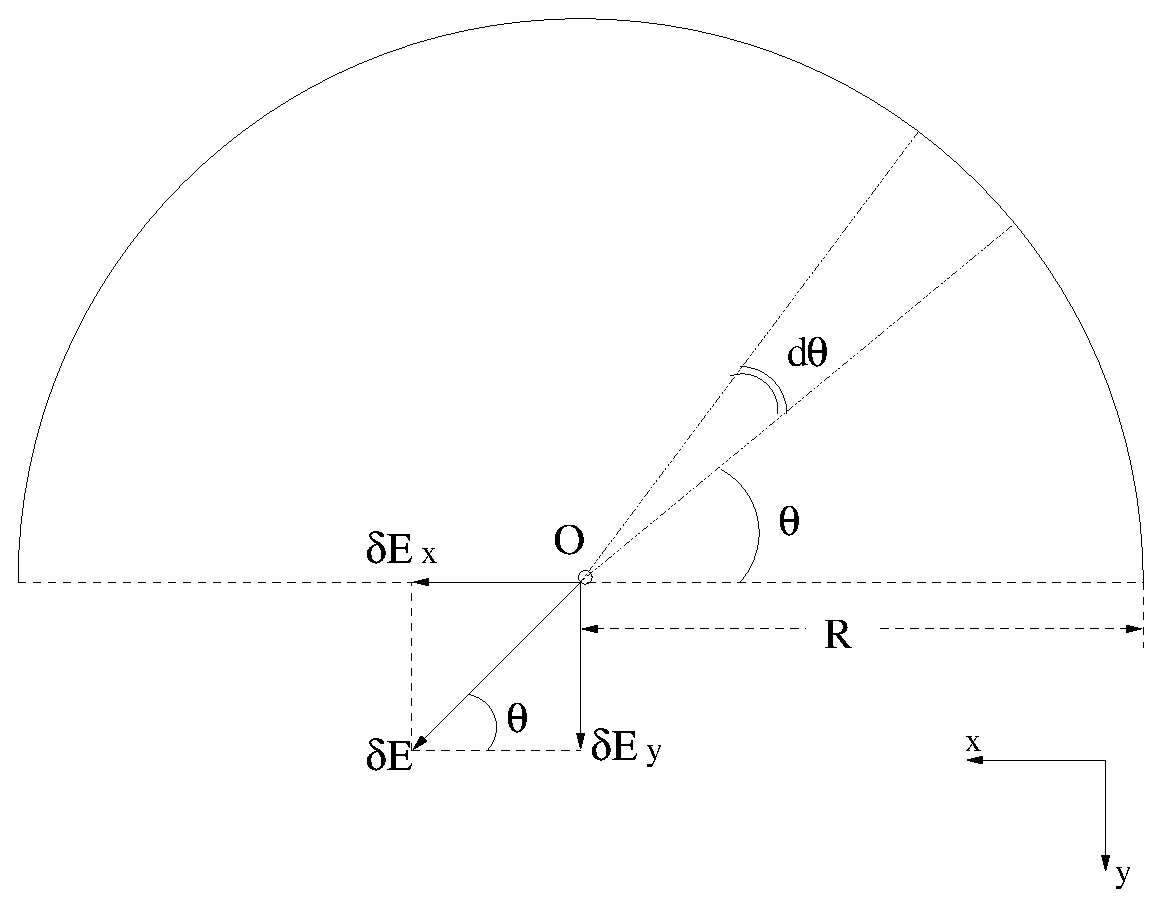
\includegraphics[width=0.5\textwidth]{ps01_sol_02}\end{center}
    \caption{A semicircular rod uniformly charged, and the contribution from an infinitesimal element arc.}
    \label{fig:problem_2}
  \end{figure}

  The total electric field at the center $O$ is the vector summation of all contributions from infinitely many pieces of element arcs on the semicircle.  \autoref{fig:problem_2} shows the contribution from one element arc that corresponds to an infinitesimal angular change of $d\theta$. The magnitude of its contribution is
  \begin{equation}\label{eq:problem_2_magnitude_delta_E}
    \delta E = \frac{\lambda (R\,d\theta)}{R^2},
  \end{equation}
  where $\lambda$ is the linear charge density of the semicircular rod,
  \begin{equation*}\label{eq:problem_2:lambda}
    \lambda = \frac{Q}{\pi R},
  \end{equation*}
  and $R\,d\theta$ is the length of the element arc. Note that in \autoref{eq:problem_2_magnitude_delta_E} we've taken $k = 1$ since $Q$ is in esu.

  One can easily observe the fact that the magnitude $\delta E$ keeps the same for ALL pieces of element arcs, since the charge is uniformly distributed. Then it is expected that the contributions for $x$-components of the field from all elements are completely canceled, while the contributions for $y$-components are added up, since we can always find a symmetric piece on the other side of a given element arc, which gives an $\delta E_x$ of opposite sign and an $\delta E_y$ of the same sign.  Therefore, the total electric field at $O$ is
  \begin{align*}
    E_O & = \sum_{\text{all pieces}} \delta E_y \\
        & = \sum_{\text{all pieces}} \delta E\sin\theta \\
        & = \int_0^\pi \frac{2Q}{\pi R^2}\sin\theta\,d\theta \\
        & = \frac{2Q}{\pi R^2}.
  \end{align*}
  The direction of $\vec E_O$ is along positive $y$-axis. Aside: one can check $E_{O,x} = \sum \delta E_x \propto \int_0^\pi \cos\theta\,d\theta = 0$.
\section{Problem \thesection: Purcell 1.8}
\subsection{Problem}
  Calculate the potential energy, per ion, for an infinite one-dimensional ionic crystal, that is, a row of equally spaced charges of magnitude $e$ and alternating sign.

  \noindent [\emph{Hint}: The power series expansion of $\ln(1+x)$,
  $$\ln(1+x) = \sum_{j=1}^\infty \frac{(-x)^{j-1}}{j},$$
  may be of use.]
\subsection{Solution}
  Let $a$ be the ionic spacing of the one-dimensional crystal. Place the first positive ion at $x = 0$, two negative ions at $x = \pm a$, two more positive ions at $x = \pm 2a$, etc.

  In class we derived that the work done in assembling an arrangement of charges is given by
  $$U = \frac12 \sum_{j=1}^N\sum_{k\ne j} \frac{q_j q_k}{r_{jk}}.$$

  We call ion 1 the charge at the origin.

  The arrangement of positive ions and negative ions is exactly the same, it doesn't matter which one we pick.

  Without loss of generality we can therefore reduce the double sum to the single sum over the interactions of ion 1 with all the others.

  $$U = \frac12 N\sum_{k=2}^N \frac{q_1 q_k}{r_{1k}},$$

  Furthermore, since the string of ions is symmetric about $x = 0$, we may consider in the single sum only the ions with $x > 0$, at the expense of multiplying the result by an extra factor of 2:

  $$U = \frac12 2N \sum_{k = 2;\ x > 0}^N \frac{q_1 q_k}{r_{1k}}.$$

  Here we evaluate $r_{1k} = a(k-1)$, and we use the fact that the sign of $q_1 q_k$ is equal to $(-1)^{k-1}$:
  \begin{align*}
    U & = \frac12 2N \sum_{k = 2}^N \frac{q_1 q_k}{a(k-1)} \\
      & = \frac{N e^2}{a} \sum_{k=2}^N \frac{(-1)^{k-1}}{k-1} \\
      & = \frac{N e^2}{a} \sum_{j=1}^{N-1} \frac{(-1)^j}{j}.
  \end{align*}
  Taking $N \to\infty$ in the limit of the sum,
  \begin{align*}
    U & = \frac{N e^2}{a} \sum_{j=1}^\infty \frac{(-1)^j}{j} \\
      & = -\frac{N e^2}{a}\ln(1 + 1) \\
    \frac{U}{N} & = -\frac{e^2}{a}\ln 2,
  \end{align*}
  where, following the hint, we have evaluated the sum by using the Taylor expansion
  $$\ln(1 + b) = \sum_{j=1}^\infty \frac{(-b)^{j-1}}{j}.$$
\section{Problem \thesection: Purcell 1.9 (next week we will solve the same problem in a different way)}
\subsection{Problem}
  A spherical volume of radius $a$ is filled with charge of uniform density $\rho$. We want to know the potential energy $U$ of this sphere of charge, that is, the work done in assembling it. Calculate it by building the sphere up layer by layer.  Express the result in terms of the total charge $Q$ in the sphere.
  \begin{flushright}\emph{Ans}. $U = \frac35 (Q^2 / a)$\end{flushright}
\subsection{Solution}
  \begin{center}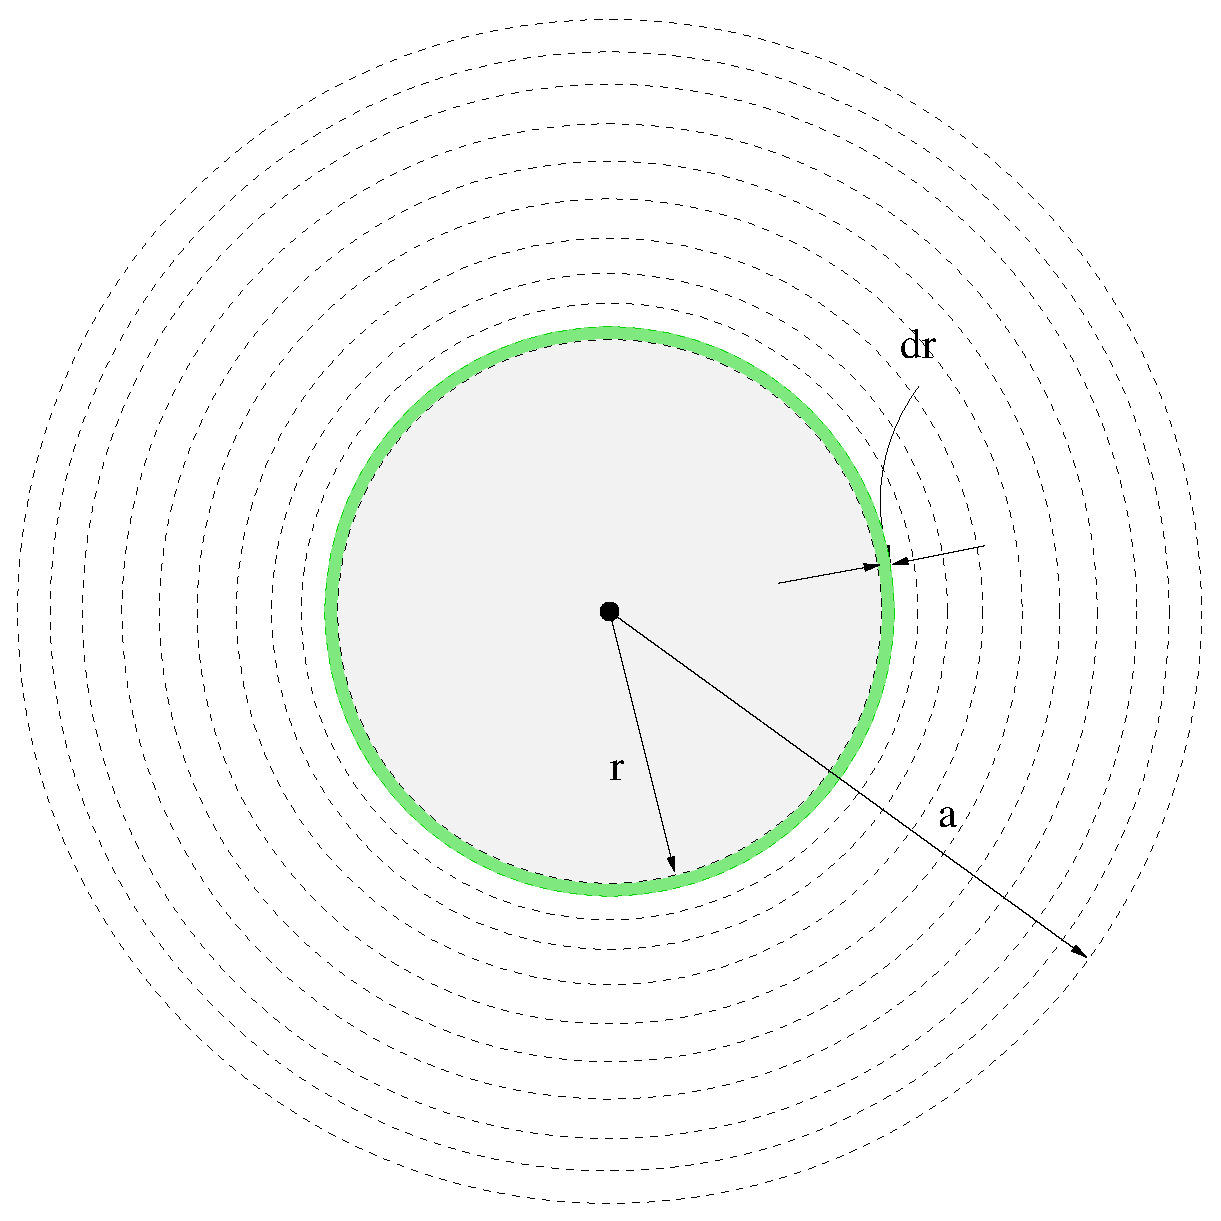
\includegraphics[width=0.4\textwidth]{ps01_sol_04}\end{center}
  \begin{center}A uniformly charged sphere, assembled layer by layer.\end{center}
  In this problem, we imagine to assemble infinitely many pieces of element charges together layer by layer around the center of sphere.  Each layer carries a charge of $\delta q = \rho\,dV$ where $\rho$ is the uniform charge density and $dV = 4\pi r^2\,dr$ the layer's volume.  Let's do it in a recursive way.  Suppose we have assembled a uniformly charged sphere of radius $r$. By putting another layer on it, the potential energy $U$ is increased by an amount
  \begin{align*}
    \delta U & = \frac{(\frac43 \rho \pi r^3)(\rho\,dV)}{r} \\
    \intertext{where we used the general expression $U = q_1 q_2 / r$, with $q_1$ being the charge of the sphere that has already being assembled, $q_2 = \delta q$.}
             & = \frac{16}{3} \pi^2 \rho^2 r^4\,dr \\
    \intertext{So, the total potential is given by}
           U & = \sum_{\text{all layers}} \delta U \\
             & = \int_0^a \frac{16}{3}\pi^2 \rho^2 r^4\,dr \\
             & = \frac{16}{15}\pi^2 \rho^2 a^5
  \end{align*}
  Note that in terms of total charge $Q$, $\rho = Q / (\frac43 \pi a^3)$. Hence the total potential is
  \begin{equation}\label{eq:problem_4}
    U = \frac{3Q^2}{5a},
  \end{equation}
  where we implicitly employ the CCS electrostatic units, i.e. the unit of $Q$ is esu. If you prefer to use SI units, a factor of $\frac{1}{4\pi \varepsilon_0}$ is added in \autoref{eq:problem_4},
  $$U = \frac{1}{4\pi \epsilon_0} \frac{3Q^2}{5a}.$$
\section{Problem \thesection: Purcell 1.11}
\subsection{Problem}
  A charge of 1 esu is at the origin. A charge of $-2$ esu is at $x = 1$ on the $x$ axis.
  \begin{enumerate}[(a)]
    \item Find a point on the $x$ axis where the electric field is zero.
    \item Locate, at least approximately, a point on the $y$ axis where the electric field is parallel to the $x$ axis.
  \end{enumerate}
\subsection{Solution}
  %\begin{enumerate}[(a)]
    %\item The electric field is zero if $\frac{(1\text{ esu})}{x^2} + \frac{(-2\text{ esu})}{(x - 1)^2} = 0$.  Then $x^2 = \frac{(x - 1)^2}{2}$, so $x\sqrt{2} = x - 1$, or $x(\sqrt{2} - 1) = -1$, so $x = \frac{1}{1 - \sqrt{2}} = -1 - \sqrt{2}$.
    %\item The electric field is $\vec E(0, y) = \frac{(1\text{ esu})\hat j}{y^2} - \frac{(2\text{ esu})(-\hat i + y\hat j)}{\sqrt{(1-0)^2 + (y-0)^2}^3} = \frac{1}{y^2}\hat j - \frac{2(-\hat i + y\hat j)}{\sqrt{1 + y^2}^3} = \left(\frac{1}{y^2} - \frac{2y}{\sqrt{1 + y^2}^3}\right)\hat j + \frac{2}{\sqrt{1 + y^2}^3}\hat i$.  For the field to be parallel to the $x$ axis, $\frac{1}{y^2} = \frac{2y}{\sqrt{1 + y^2}^3}$, so $2y^3 = \sqrt{1 + y^2}^3$, or $y^2\sqrt[3]{2} = 1 + y^2$.  Then $y^2(\sqrt[3]{2} - 1) = 1$, or $y = \pm \frac{1}{\sqrt{\sqrt[3]{4} - 1}}$.
  %\end{enumerate}
  \begin{center}\includegraphics[width=0.2\textwidth]{ps01_sol_05}\end{center}
  \begin{enumerate}[(a)]
    \item The field $E$ cannot be zero anywhere \emph{between} two charges of opposite sign, or at any point closer to the greater than to the lesser charge. Hence the point we seek must lie on the negative $x$-axis. It is well to be clear about this before plunging into algebra. Let the point lie at $x = -s$. The field will vanish there if $1 / x^2 = 2 / (1+s)^2$, giving us the quadratic equation $s^2 - 2s - 1 = 0$, with roots $s = 1 \pm \sqrt{2}$. The positive root locates the point of vanishing field at $x = -2.414$.  What is wrong with the other root?
    \item At $(0, y)$ the field component $E_y$ has the value $\frac{1}{u^2} - \frac{2}{(1 + y^2)^{3/2}}$.  This vanishes if $2y^3 = (1 + y^2)^{3/2}$ which can be written $2^{2/3}y^2 = 1 + y^2$, giving $y = \frac{1}{\sqrt{\sqrt[3]{4} - 1}} = 1.305$.
  \end{enumerate}
\section{Problem \thesection: Purcell 1.12}
\subsection{Problem}
  Two positive ions and one negative ion are fixed at the vertices of an equilateral triangle.  Where can a fourth ion be placed so that the force on it will be zero?  Is there more than one such place?

  Note, the ions all have the same \emph{magnitude} of charge, i.e., the charges are $+Q$, $+Q$, and $-Q$. You may consider only solutions that lie on the axis of symmetry. Are there other possible solutions?

  \textsc{Optional}: Use Mathematica (\url{http://ist.mit.edu/services/software/mathematica/obtain}) or Wolfram Alpha (\url{http://www.wolframalpha.com/}) to solve the final equation.
\subsection{Solution}
  \begin{center}\includegraphics[width=0.3\textwidth]{ps01_sol_06}\end{center}
  We will look for a point on the line passing through $A$ and the origin $(O)$, where the electric field is zero (see the figure above). We will also assume that the length of each side of the equilateral triangle is $2a$. The electric field of a charge distribution at the point $(x, y, z)$ is given by (in CGS units)
  \begin{equation*}
    \vec E(x,y,z) = \sum_{j = 1}^3 \frac{q_j \vec r_{0j}}{\vec r_{0j}^2}.
  \end{equation*}
  The electric field at point $P = (0, h)$ produced by the charge $A$ is
  \begin{equation*}
    \vec E_A(h) = -Q\frac{(h - \sqrt3 a)\hat y}{|h - \sqrt3 a|^3},
  \end{equation*}
  the one produced by charge $B$ is
  \begin{align*}
    \vec E_B(h) & = Q\frac{1}{h^2 + a^2} \left(\frac{h\hat y}{\sqrt{h^2 + a^2}} + \frac{a\hat x}{\sqrt{h^2 + a^2}}\right) \\
                & = Q\frac{h\hat y + a\hat x}{(h^2 + a^2)^{3/2}}
  \end{align*}
  and finally the one from charge $C$
  \begin{equation*}
    \vec E_C(h) = Q\frac{h\hat y - a\hat x}{(h^2 + a^2)^{3/2}}
  \end{equation*}
  The total electric field at $P = (0, 0, h)$, is given by the sum of the three electric fields produced by each charge, so
  \begin{align*}
    \vec E(h) & = Q\left(\frac{h\hat y - a\hat x}{(h^2 + a^2)^{3/2}} + \frac{h\hat y + a\hat x}{(h^2 + a^2)^{3/2}} - \frac{(h - \sqrt3 a)\hat y}{|h - \sqrt3 a|^3}\right) \\
              & = Q\hat y\left(\frac{2h}{(h^2 + a^2)^{3/2}} - \frac{(h - \sqrt3 a)}{|h - \sqrt3 a|^3}\right)
  \end{align*}
  The force on the fourth ion is zero if the charge is placed at the point where electric field vanishes. This happens when
  \begin{equation*}
    \frac{2h}{(h^2 + a^2)^{3/2}} - \frac{(h - \sqrt3 a)}{|h - \sqrt3 a|^3} = 0
  \end{equation*}
  The above equation can be solved using \texttt{NSolve}, or \texttt{N} and \texttt{Reduce}, in Mathematica\footnote{$N\left[\text{Reduce}\left[\frac{2 h}{\left(h^2+a^2\right)^{3/2}}-\frac{h-\sqrt{3}a}{\left(\text{Abs}\left[h-\sqrt{3}a\right]\right)^3}==0\&\&\text{hoa}\text{==}h/ a,\{\text{hoa},h\},\text{Reals}\right]\right]\text{/.}\text{hoa}\to h/a$}, or via Wolfram Alpha\footnote{Define $H$ as $h / a$, replace $h$ by $H a$, and simplify the equation to remove the $a$s, then put \texttt{(2 h)/((h)$\wedge$2 + 1)$\wedge$(3/2) - (h - Sqrt[3])/(Abs[h - Sqrt[3]])$\wedge$3 = 0} into Wolfram Alpha.}. There are 2 roots for the above equation
  $$h_- = -0.1462a;\ h_+ = 6.204a$$
  Hence, the force vanishes at $(0, h_-)$ and $(0, h_+)$. There is more than one choice to place the fourth ion in such a way that it experiences zero force.
\section{Problem \thesection: Electric Dipole}
\subsection{Problem}
  A pair of charges lie in the $xy$-plane.  The charge $q$ is at coordinate $x = 0$, $y = b$; the charge $-q$ is at coordinate $x = 0$, $y = -b$.
  \begin{center}\includegraphics[width=0.2\textwidth]{ps01_8}\end{center}
  \begin{enumerate}[(a)]
    \item Evaluate the electric field (magnitude \emph{and} direction) on the $x$-axis.  Show that for $x \gg b$, $|\vec E| \propto 1 / x^3$.  What is the direction in this limit?
    \item Evaluate the electric field on the $y$-axis.  Consider $y < -b$, $-b < y < b$, and $b < y$ separately.  Additionally, find the magnitude and direction for $y \gg b$.
  \end{enumerate}
\subsection{Solution}
  Electric dipole - we will come back to this with a different approach
  \begin{center}\includegraphics[width=0.9\textwidth]{ps01_sol_07_1}\end{center}
  \begin{center}\includegraphics[width=0.9\textwidth]{ps01_sol_07_2}\end{center}
\section{Problem \thesection: Coulomb force between line charges}
\subsection{Problem}
  A rod of length $l_1$ with linear charge density $\lambda_1$ and a rod of length $l_2$ with linear charge density $\lambda_2$ lie on the $x$-axis.  Their ends are separated by a distance $D$ as shown in the figure.
  \begin{center}\includegraphics[width=0.4\textwidth]{ps01_9}\end{center}
  Assume that the charge densities have the same sign.
  \begin{enumerate}[(a)]
    \item What is the force $\vec F$ between these charges?
    \item Show that for $D \gg l_1$ and $D \gg l_2$, this force reduces to the Coulomb forces between a pair of point charges, $q_1 = l_1\lambda_1$, $q_2 = l_2\lambda_2$.
  \end{enumerate}
\subsection{Solution}
  \begin{enumerate}[(a)]
    \item It's convenient to set up two coordinates for rod 1 and rod 2, shown in the figure below, in which axis $x_1$ originates from its right end and extends towards the left, and axis $x_2$, originates from its left end and extends towards the right.  Pick up two clement charges $dx_1$, and $dx_2$. The force between them is repulsive, and the magnitude is
    \begin{equation*}
      \delta F = \frac{(\lambda_1\,dx_1)(\lambda_2\,dx_2)}{(x_1 + x_2 + D)^2}.
    \end{equation*}
    \begin{center}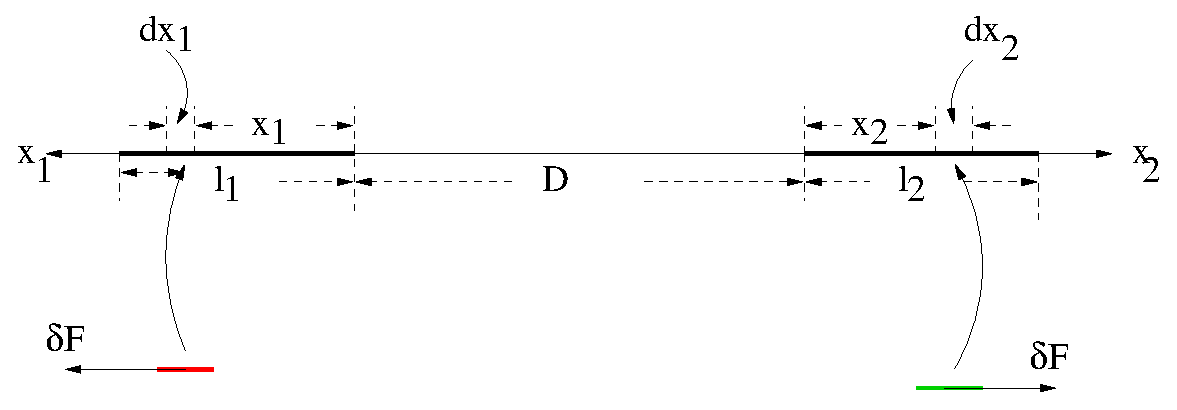
\includegraphics[width=0.5\textwidth]{ps01_sol_08}\end{center}
    \begin{center}Electric field of a pair of line charges.\end{center}
    The force between rod 1 and rod 2 is the sum over all pieces of element charges.
    \begin{align*}
      F & = \int_0^{l_1}dx_1\int_0^{l_2}dx_2\frac{\lambda_1\lambda_2}{(x_1 + x_2 + D)^2} \\
        & \lambda_1 \lambda_2 \log\frac{(D + l_1)(D + l_2)}{D(D + l_1 + l_2)}.
    \end{align*}
    The force $\vec F$ is repulsive, i.e. the force on rod 1 is to the left and that on rod 2 to the right.
  \item When $D \gg l_1$ and $D \gg l_2$,
    \begin{align*}
      \log\frac{(D + l_1)(D + l_2)}{D(D + l_1 + l_2)} & = \log(1 + \frac{l_1}{D}) - \log(1 + \frac{l_1}{D + l_2}) \\
        & \approx \frac{l_1}{D} - \frac12 \left(\frac{l_1}{D}\right)^2 - \frac{l_1}{D + l_2} + \frac12 \left(\frac{l_1}{D + l_2}\right)^2 + \mathcal O\left(\frac{l_1}{D}\right) \\
        & \approx \frac{l_1}{D} - \frac12\left(\frac{l_1}{D}\right)^2 - \frac{l_1}{D}(1 - \frac{l_2}{D}) + \frac12 \left(\frac{l_1}{D}\right)^2 + \mathcal O\left(\frac{l_1}{D}\right)^3 \\
        & = \frac{l_1 l_2}{D^2} + \mathcal O\left(\frac{l_1}{D}\right)^3
    \end{align*}
    where we used the approximation that $\log(1 + x) = x - \frac12x^2 + \cdots$ and $(1 + x)^n = 1 + nx + \cdots$ for $x \ll 1$ so that
    \begin{align*}
      \frac{l_1}{D + l_2} & = \frac{l_1}{D}(1 + \frac{l_2}{D})^{-1} \\
        & \approx \frac{l_1}{D}(1 - \frac{l_2}{D}) \\
      \frac12 \left(\frac{l_1}{D + l_2}\right)^2 & = \frac12 \left(\frac{l_1}{D}\right)^2(1 - \frac{l_2}{D})^2 \\
        & = \frac12 \left(\frac{l_1}{D}\right)^2(1 - \frac{2l_2}{D}) \\
        & = \frac12 \left(\frac{l_1}{D}\right)^2 + \mathcal O\left(\frac{l_1}{D}\right)^3
    \end{align*}
    Therefore the force reduces to be
    \begin{align*}
      F & = \frac{\lambda_1 \lambda_2 l_1 l_2}{D^2} \\
        & = \frac{q_1 q_2}{D^2}
    \end{align*}
    where $q_1 = l_1\lambda_1$, $q_2 = l_2\lambda_2$.  Thus the force turns to be that between a pair of point charges $q_1$ and $q_2$.
  \end{enumerate}
\end{document}
